\section{So sánh hiệu năng}
So sánh hiệu năng (thời gian thực thi) và độ chính xác của hai thuật toán nhân: \textit{Linear Multiply} và \textit{Fast Multiply}, khi được thực hiện trên hai kiểu dữ liệu \texttt{float(32 bit)} (độ chính xác đơn) và \texttt{double(64 bit)} (độ chính xác kép). Dữ liệu được lấy từ kết quả benchmark với các giá trị $n$ từ 10 đến 100,000,000,000 và $x=0.1$\\

Bài so sánh này được thực hiện bằng ngôn ngữ lập trình C++.

\subsection{Kết quả so sánh}
\begin{landscape}
\begin{table}
    \centering
    \caption{Kết quả benchmark cho kiểu dữ liệu \texttt{float} }
    \small % Giảm kích thước chữ
    \begin{tabular}{r r r r r r r r}
        \toprule
        $n$ & Linear Result & Fast Result & Expected & Linear Error (\%) & Fast Error (\%)s & Linear Time (ms) & Fast Time (ms) \\
        \midrule
        10 & 1.0000001192 & 1.0000000000 & 1.0 & 0.0000001192 & 0.0000000000 & 0.1250 & 0.2080 \\
        100 & 10.0000019073 & 10.0000000000 & 10.0 & 0.0000001907 & 0.0000000000 & 1.1670 & 0.2080 \\
        1,000 & 99.9990463257 & 100.0000000000 & 100.0 & 0.0000095367 & 0.0000000000 & 10.5000 & 0.2500 \\
        10,000 & 999.9028930664 & 1000.0000000000 & 1000.0 & 0.0000971069 & 0.0000000000 & 104.0000 & 0.2920 \\
        100,000 & 9998.5566406250 & 10000.0000000000 & 10000.0 & 0.0001443359 & 0.0000000000 & 1041.8330 & 0.3330 \\
        1,000,000 & 100958.3437500000 & 100000.0000000000 & 100000.0 & 0.0095834378 & 0.0000000000 & 9578.3330 & 0.6670 \\
        10,000,000 & 1087937.0000000000 & 1000000.0000000000 & 1000000.0 & 0.0879369974 & 0.0000000000 & 51153.9580 & 0.2500 \\
        100,000,000 & 2097152.0000000000 & 10000000.0000000000 & 10000000.0 & 0.7902848125 & 0.0000000000 & 358622.3750 & 0.5000 \\
        1,000,000,000 & 2097152.0000000000 & 100000000.0000000000 & 100000000.0 & 0.9790284634 & 0.0000000000 & 3605166.4580 & 0.2920 \\
        10,000,000,000 & 2097152.0000000000 & 1000000000.0000000000 & 1000000000.0 & 0.9979028702 & 0.0000000000 & 35451535.1670 & 0.3750 \\
        100,000,000,000 & 2097152.0000000000 & 10000000000.0000000000 & 10000000000.0 & 0.9997903109 & 0.0000000000 & 349873786.2500 & 0.5410 \\
        \bottomrule
    \end{tabular}
\end{table}

\begin{table}
    \centering
    \caption{Kết quả benchmark cho kiểu dữ liệu \texttt{double}}
    \small % Giảm kích thước chữ
    \begin{tabular}{r r r r r r r r}
        \toprule
        $n$ & Linear Result & Fast Result & Expected & Linear Error & Fast Error & Linear Time (ms) & Fast Time (ms) \\
        \midrule
        10 & 1.0000000000 & 1.0000000000 & 1.0 & 0.0000000000 & 0.0000000000 & 0.0000 & 0.0830 \\
        100 & 10.0000000000 & 10.0000000000 & 10.0 & 0.0000000000 & 0.0000000000 & 0.3750 & 0.0830 \\
        1,000 & 100.0000000000 & 100.0000000000 & 100.0 & 0.0000000000 & 0.0000000000 & 3.5000 & 0.0830 \\
        10,000 & 1000.0000000002 & 1000.0000000000 & 1000.0 & 0.0000000000 & 0.0000000000 & 35.2500 & 0.1250 \\
        100,000 & 10000.0000000188 & 10000.0000000000 & 10000.0 & 0.0000000000 & 0.0000000000 & 366.0840 & 0.1670 \\
        1,000,000 & 100000.0000013329 & 100000.0000000000 & 100000.0 & 0.0000000000 & 0.0000000000 & 3454.6670 & 0.1250 \\
        10,000,000 & 999999.9998389754 & 1000000.0000000000 & 1000000.0 & 0.0000000002 & 0.0000000000 & 35304.9160 & 0.3750 \\
        100,000,000 & 9999999.9811294507 & 10000000.0000000000 & 10000000.0 & 0.0000000019 & 0.0000000000 & 360873.2080 & 0.3750 \\
        1,000,000,000 & 99999998.7454178184 & 100000000.0000000000 & 100000000.0 & 0.0000000125 & 0.0000000000 & 3517857.0410 & 0.4160 \\
        10,000,000,000 & 1000000163.1244580746 & 1000000000.0000000000 & 1000000000.0 & 0.0000001631 & 0.0000000000 & 35160741.7080 & 0.4170 \\
        100,000,000,000 & 10000018871.6645336151 & 10000000000.0000000000 & 10000000000.0 & 0.0000018872 & 0.0000000000 & 349189730.7920 & 0.4170 \\
        \bottomrule
    \end{tabular}
\end{table}
\end{landscape}

\subsection{So sánh độ chính xác}
Tất cả các kết quả tính toán bằng \textit{Fast Multiply} đều cho ra độ chính xác cao hơn đáng kể so với \textit{Linear Multiply}. Cụ thể, trong khi \textit{Fast Multiply} duy trì sai số gần như bằng 0 trong mọi trường hợp, \textit{Linear Multiply} lại xảy ra sai số lớn khi $n$ tăng cao, đặc biệt trên cả hai kiểu dữ liệu \texttt{float} và \texttt{double}. Nguyên nhân chủ yếu đến từ hai yếu tố sau:

Thứ nhất, với \textit{Linear Multiply}, số lượng phép tính tăng tuyến tính theo $n$, dẫn đến việc làm tròn lặp đi lặp lại nhiều lần, gây tích lũy sai số đáng kể. Ngược lại, \textit{Fast Multiply} chỉ yêu cầu $\log(n)$ lần tính toán, giúp giảm thiểu số lần làm tròn và hạn chế sai số phát sinh.

Thứ hai, trong kiểu dữ liệu \texttt{float}, \textit{Linear Multiply} gặp hiện tượng "kẹt số", khi kết quả không tăng thêm sau khi cộng thêm $x$. Đặc biệt, từ $n \geq 100,000,000$, giá trị bị cố định ở $2097152 = 2^{21}$ do giới hạn độ chính xác của \texttt{float}. Trong khi đó, \texttt{double} với độ chính xác cao hơn vẫn chịu ảnh hưởng từ sai số tích lũy, dù ít nghiêm trọng hơn so với \texttt{float}.
\begin{figure}[h]
    \centering
    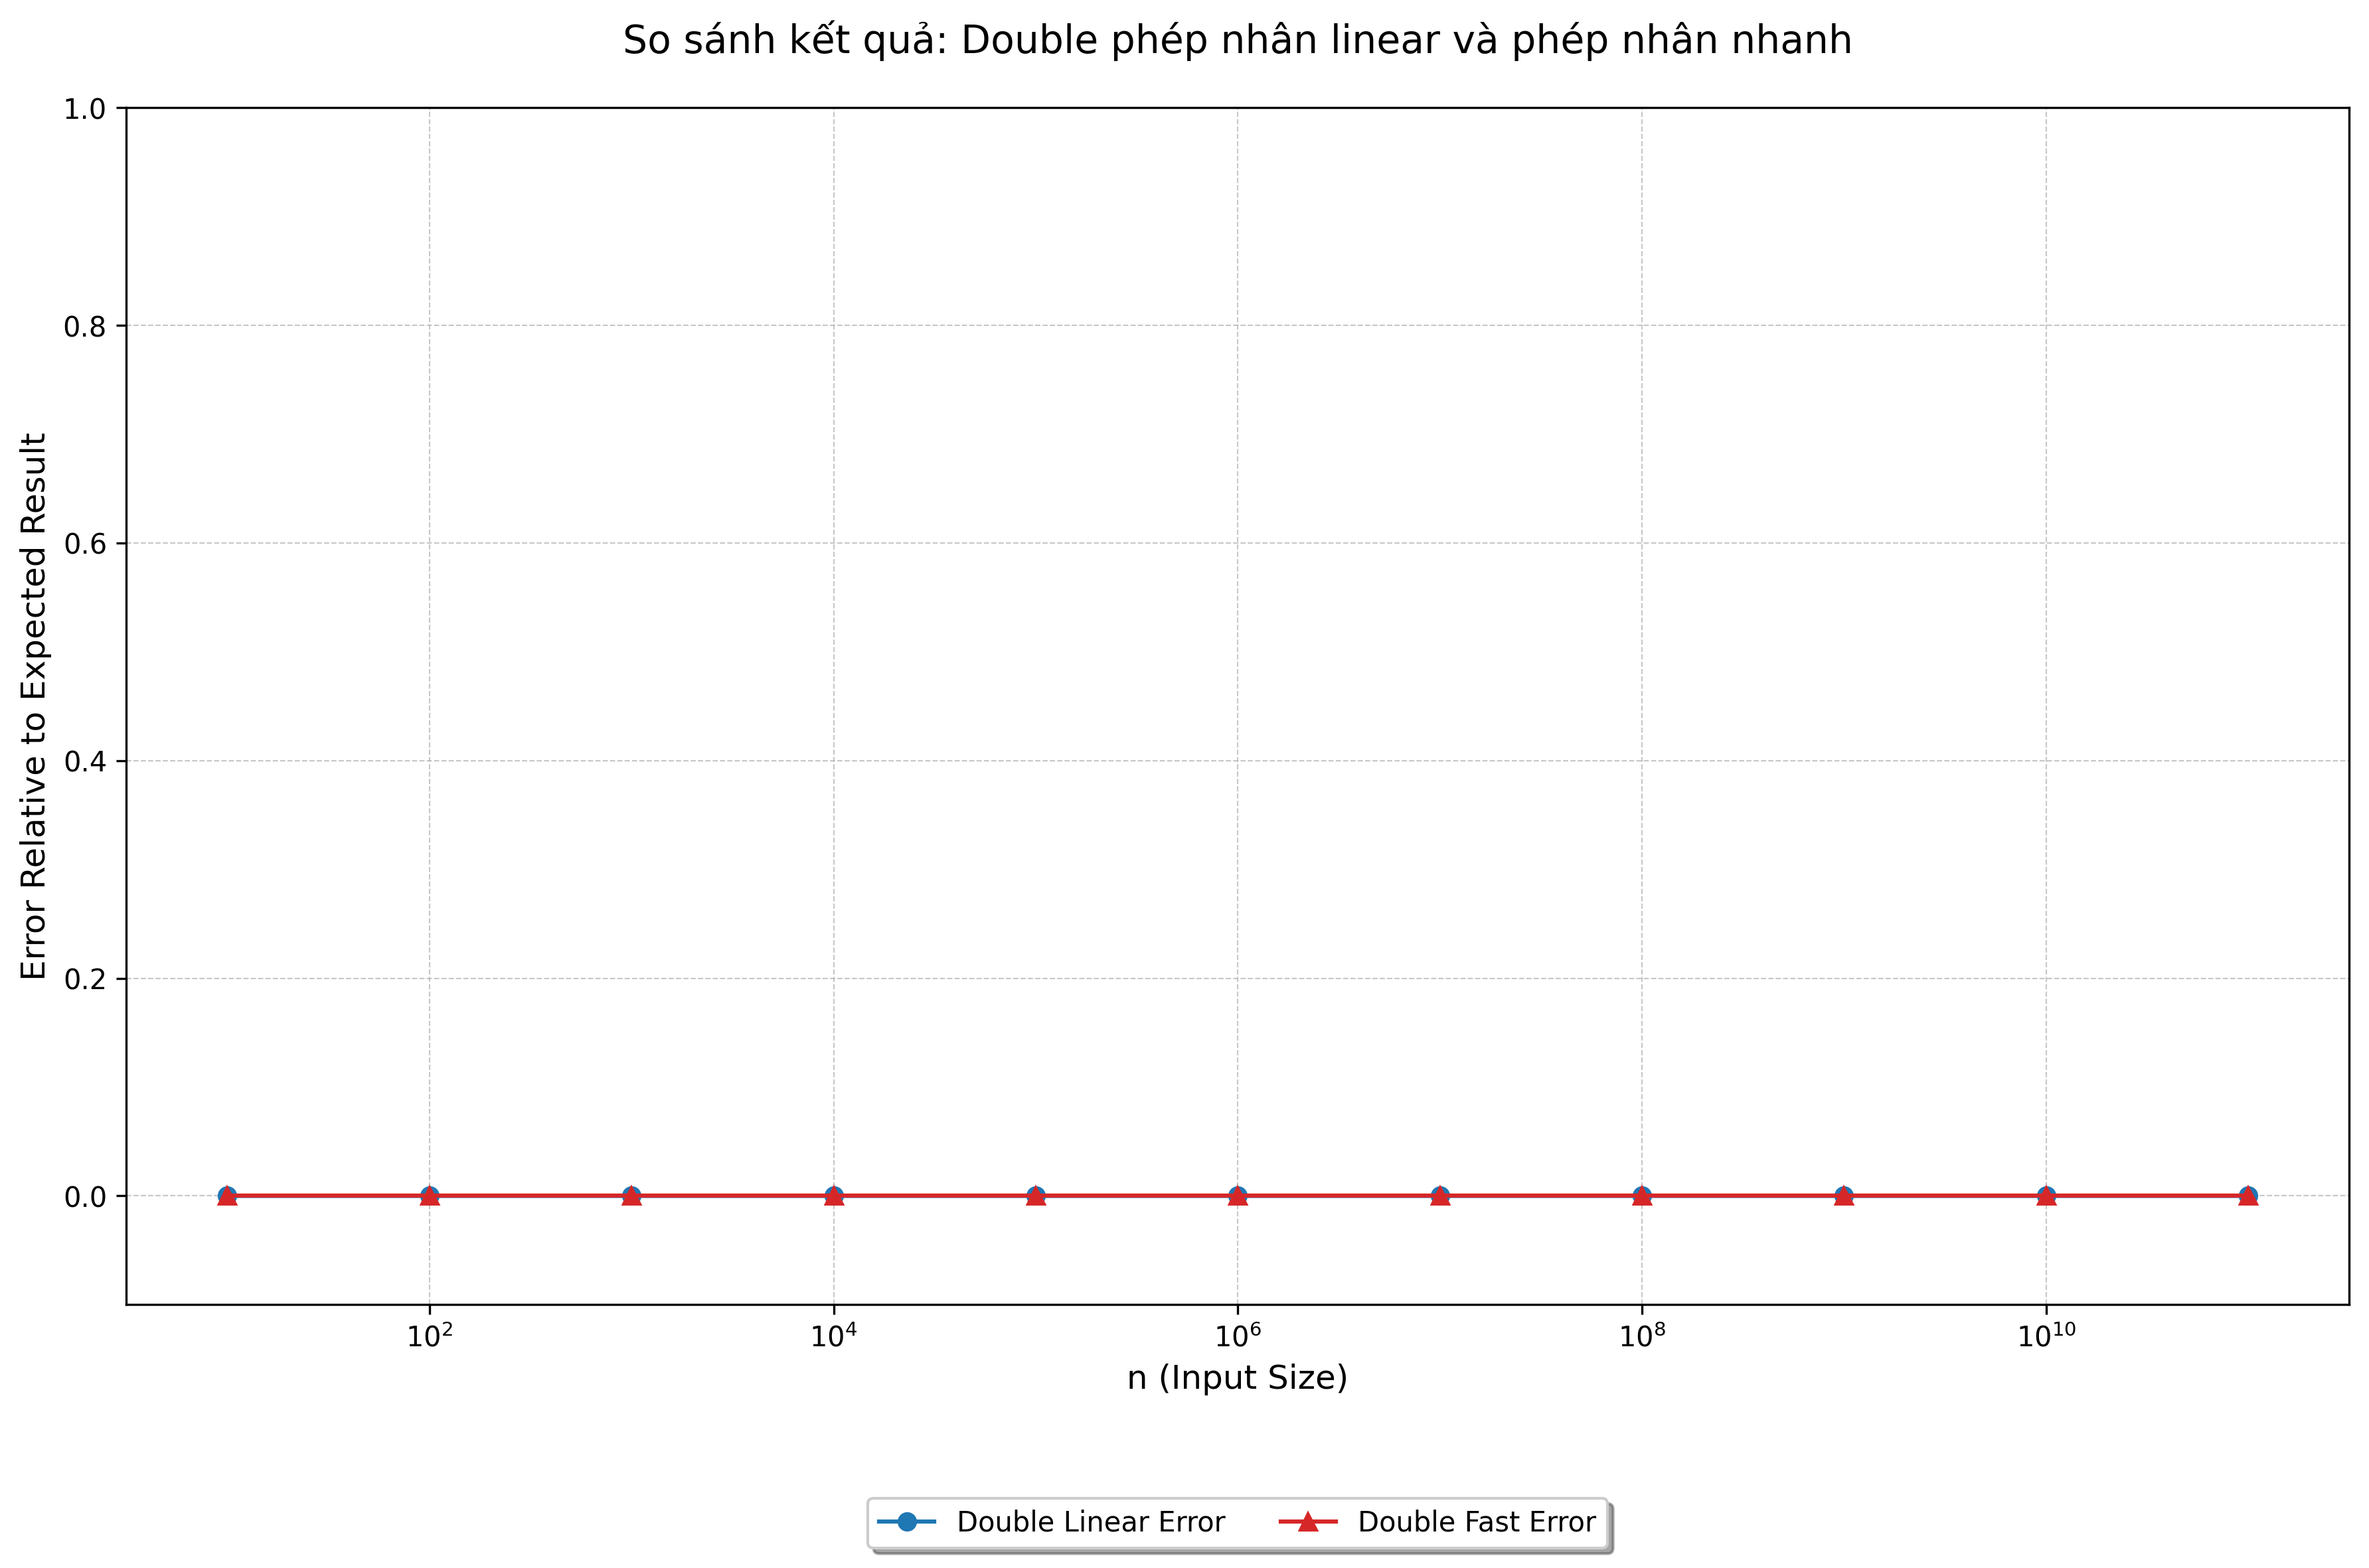
\includegraphics[width=0.7\linewidth]{images/double-percision.png}
    \caption{Kết quả so sánh về độ chính xác double}
\end{figure}
\begin{figure}[h]
    \centering
    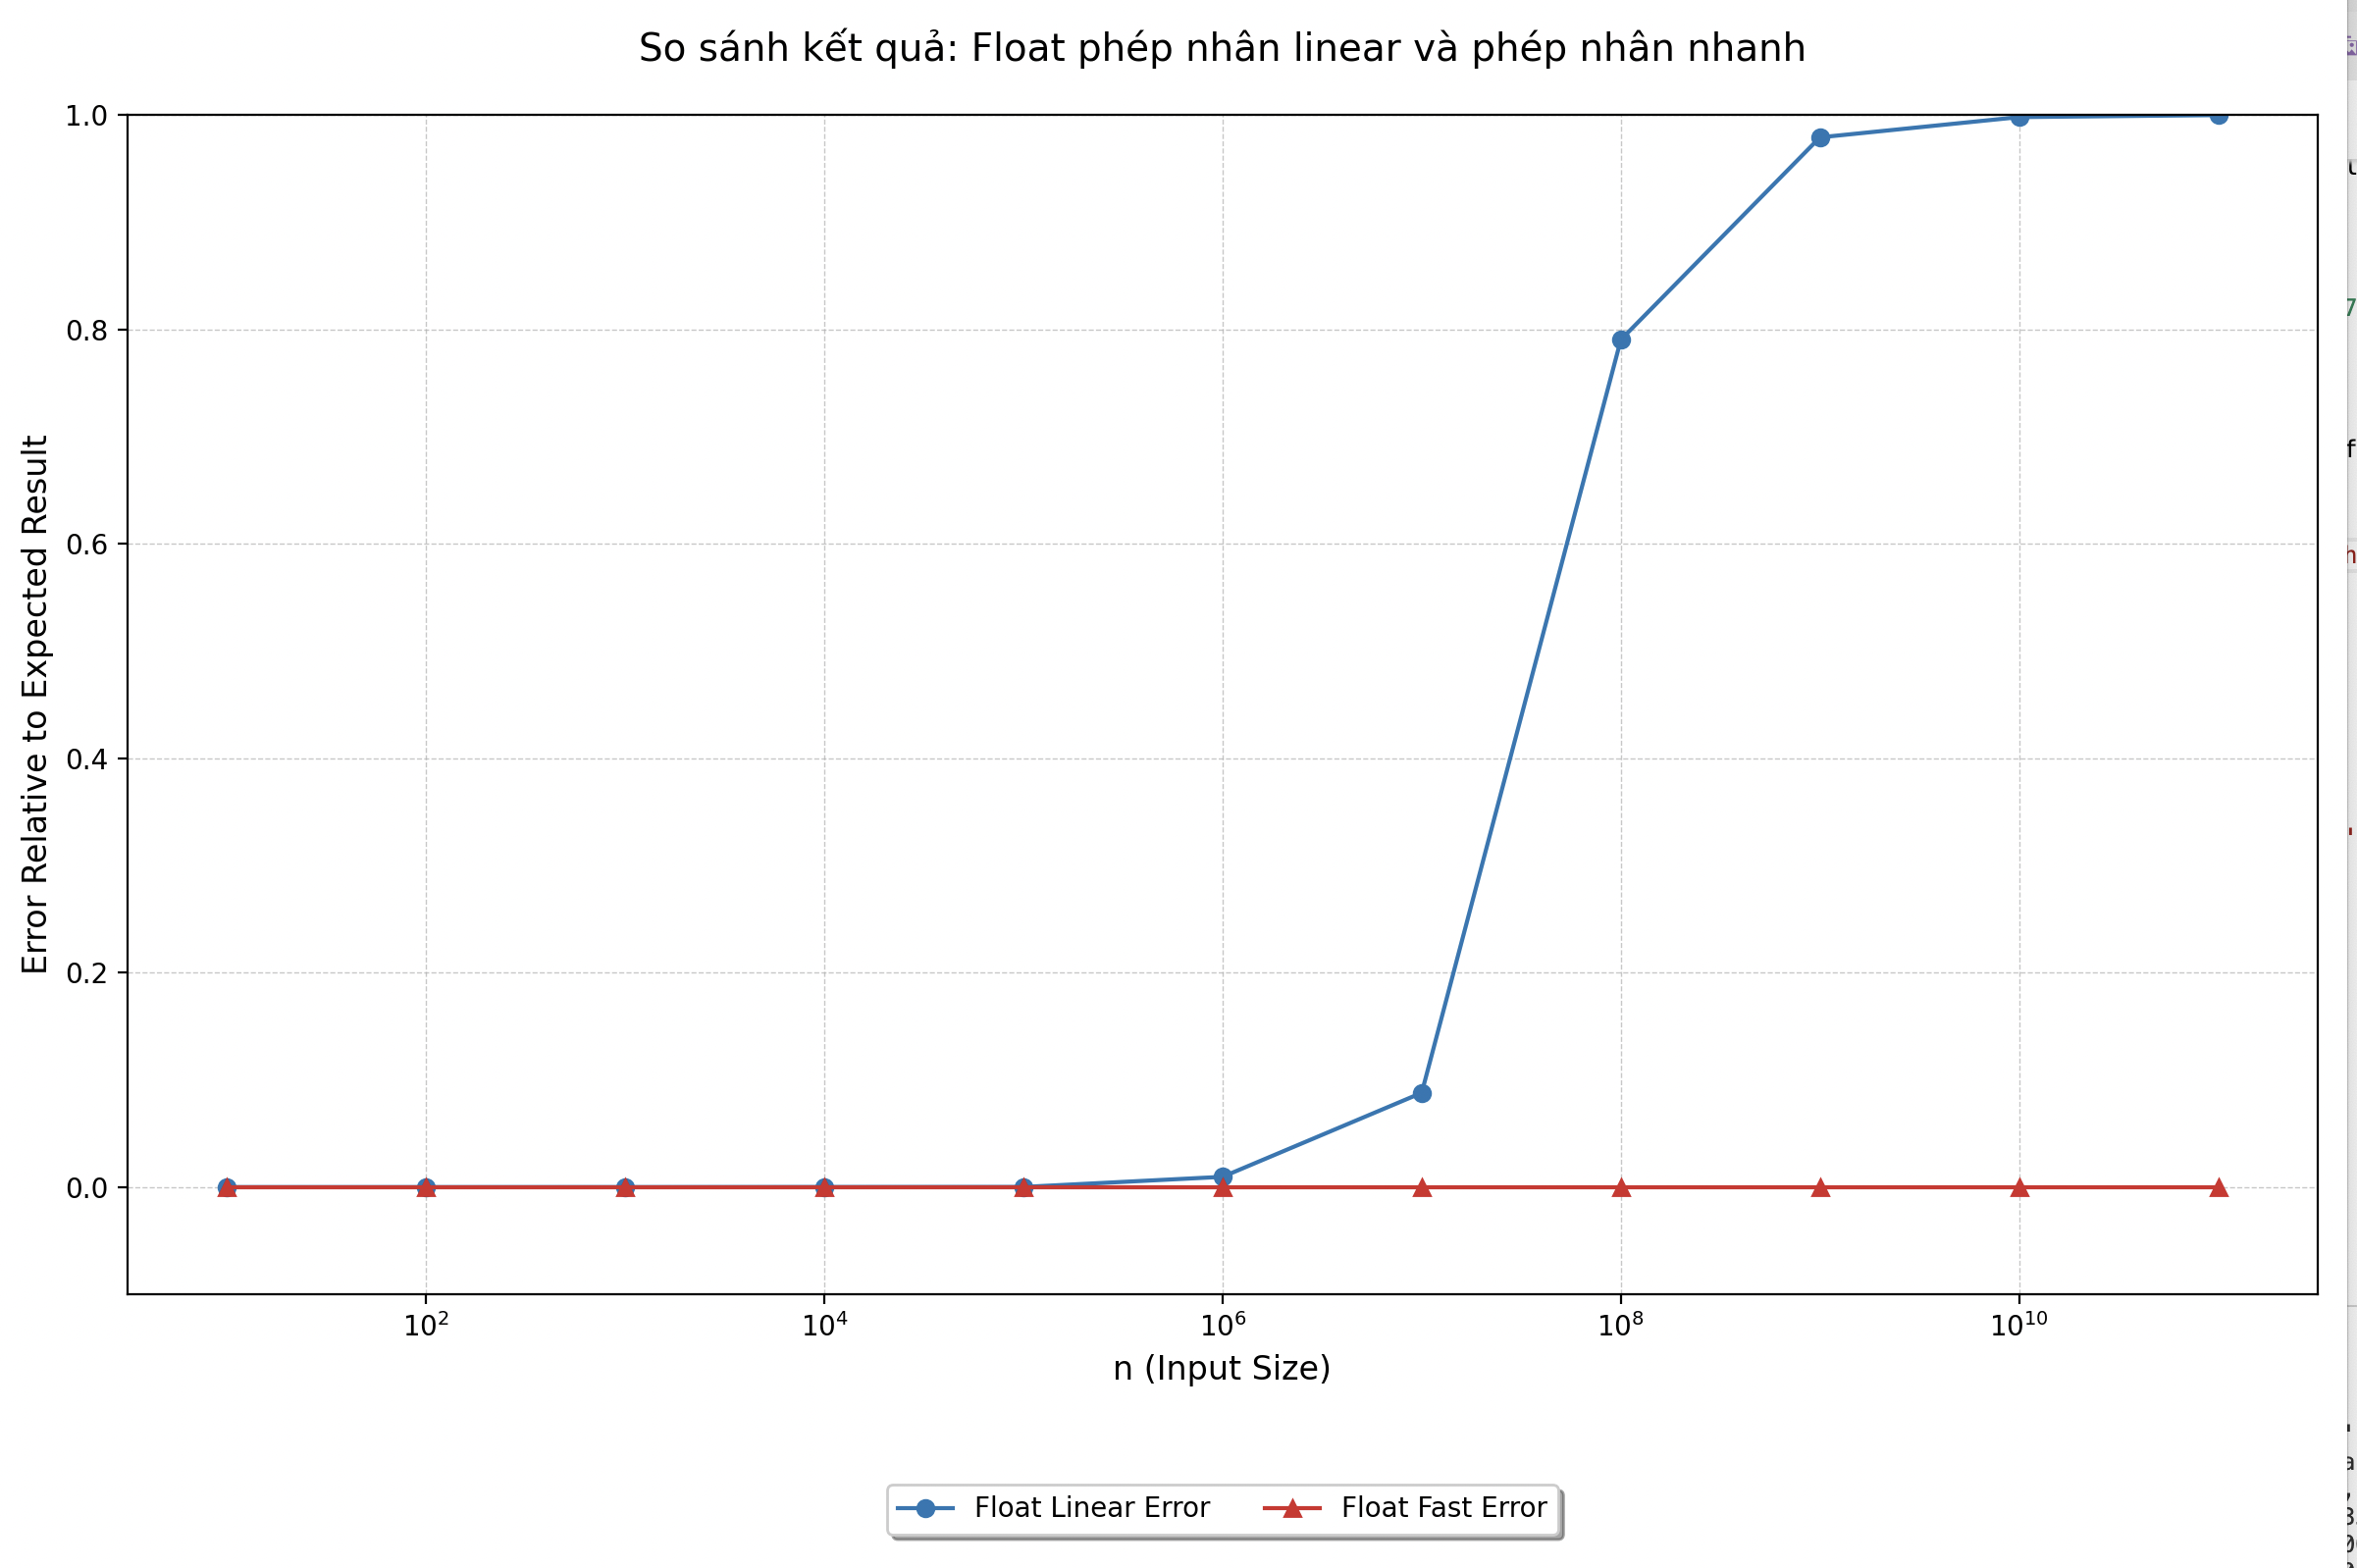
\includegraphics[width=0.7\linewidth]{images/float-percision.png}
    \caption{Kết quả so sánh về độ chính xác float}
\end{figure}

\subsection{So sánh thời gian thực thi}

\subsubsection{Độ phức tạp tính toán}
Thuật toán \textit{Linear Multiply} có độ phức tạp tính toán là $O(n)$, nghĩa là thời gian thực thi tăng tuyến tính theo kích thước đầu vào $n$. Trong khi đó, thuật toán \textit{Fast Multiply} có độ phức tạp là $O(\log n)$, cho thấy thời gian thực thi chỉ tăng theo logarit của $n$, giúp nó xử lý các giá trị lớn hiệu quả hơn nhiều so với \textit{Linear Multiply}.

\subsubsection{Đối với kiểu dữ liệu \texttt{float}}
Dựa trên kết quả benchmark:
\begin{itemize}
    \item \textbf{Tổng thời gian thực thi:}
    \begin{itemize}
        \item \textit{Linear Multiply}: 389,351.013 ms (389.351013 giây)
        \item \textit{Fast Multiply}: 0.003958 ms (0.000003958 giây)
    \end{itemize}
    \item \textbf{Tỷ lệ tốc độ:} \textit{Linear Multiply} chậm hơn \textit{Fast Multiply} khoảng $98,341,311$ lần. Sự khác biệt này phản ánh rõ ràng độ phức tạp $O(n)$ của \textit{Linear Multiply}, khi thời gian tăng mạnh với $n$, trong khi $O(\log n)$ của \textit{Fast Multiply} giữ thời gian gần như không đổi.
    \item \textbf{Thời gian trung bình mỗi phép toán:}
    \begin{itemize}
        \item \textit{Linear Multiply}: 35,395.5466 ms (35.3955466 giây)
        \item \textit{Fast Multiply}: 0.0003598 ms (gần bằng 0 giây)
    \end{itemize}
\end{itemize}

Khi $n$ tăng từ 10 lên 100,000,000,000, thời gian thực thi của \textit{Linear Multiply} tăng từ 0.1250 ms lên 349,873,786.2500 ms (gấp khoảng 2.8 triệu lần), trong khi \textit{Fast Multiply} chỉ tăng từ 0.2080 ms lên 0.5410 ms (gấp khoảng 2.6 lần), phù hợp với dự đoán từ $O(n)$ và $O(\log n)$.

\subsubsection{Đối với kiểu dữ liệu \texttt{double}}
Dựa trên kết quả benchmark:
\begin{itemize}
    \item \textbf{Tổng thời gian thực thi:}
    \begin{itemize}
        \item \textit{Linear Multiply}: 388,268.367 ms (388.268367 giây)
        \item \textit{Fast Multiply}: 0.002666 ms (0.000002666 giây)
    \end{itemize}
    \item \textbf{Tỷ lệ tốc độ:} \textit{Linear Multiply} chậm hơn \textit{Fast Multiply} khoảng $145,611,013$ lần. Tương tự như với \texttt{float}, độ phức tạp $O(n)$ khiến \textit{Linear Multiply} kém hiệu quả hơn nhiều so với $O(\log n)$ của \textit{Fast Multiply}.
    \item \textbf{Thời gian trung bình mỗi phép toán:}
    \begin{itemize}
        \item \textit{Linear Multiply}: 35,297.1243 ms (35.2971243 giây)
        \item \textit{Fast Multiply}: 0.0002424 ms (gần bằng 0 giây)
    \end{itemize}
\end{itemize}

Với \texttt{double}, thời gian của \textit{Linear Multiply} tăng từ 0.0000 ms ($n=10$) lên 349,189,730.7920 ms ($n=100$ tỷ), trong khi \textit{Fast Multiply} chỉ tăng từ 0.0830 ms lên 0.4170 ms, một lần nữa minh chứng cho ưu thế của $O(\log n)$ so với $O(n)$.
\section{Lý giải hiện tượng kẹt giá trị trong kiểu dữ liệu \texttt{float}}
Dựa vào kết quả trong bảng 1, ta có thể thấy khi $n$ đạt giá trị $100000000$ thì kết quả không tăng mà đứng lại ở giá trị $2097152 = 2^{21}$. Phần này sẽ lý giải nguyên nhân của hiện tượng trên.
\subsection{Cơ chế biểu diễn số thực trong chuẩn IEEE 754}
Trong kiểu dữ liệu \texttt{float} (32 bit), các giá trị được biểu diễn theo chuẩn IEEE 754 với 1 bit dấu (sign), 8 bit mũ (exponent) và 23 bit phần định trị (mantissa). Khi giá trị đạt tới $2097152 = 2^{21}$, biểu diễn của nó trong chuẩn IEEE 754 là:

\begin{itemize}
    \item \textbf{Dấu (Sign):} $+1$ (bit 0)
    \item \textbf{Mũ (Exponent):} $2^{21}$ (10010100)
    \item \textbf{Phần định trị (Mantissa):} $1.0$ (bit ẩn 1, các bit còn lại là 0)
\end{itemize}

Cụ thể, dạng nhị phân của $2097152$ là: \texttt{01001010 00000000 00000000 00000000}.\\
Số lớn hơn liền kề trong biểu diễn \texttt{float} là: \texttt{01001010 00000000 00000000 00000001}, tương ứng với:
\begin{itemize}
    \item \textbf{Dấu (Sign):} $+1$
    \item \textbf{Mũ (Exponent):} $2^{21}$
    \item \textbf{Phần định trị (Mantissa):} $1 + 2^{-23} \approx 1 + 0.00000011920928955078125$
\end{itemize}

Khi chuyển sang hệ thập phân, giá trị này là $2097152.25$. Khoảng cách giữa $2097152$ và số lớn hơn gần nhất là $0.25$, do giới hạn độ chính xác của 23 bit mantissa trong \texttt{float}.\\ \\ 
Vì vậy, khi thực hiện phép tính $2097152 + 0.1 = 2097152.1$, kết quả nằm giữa $2097152$ và $2097152.25$. Theo quy tắc làm tròn của IEEE 754 (thường là làm tròn xuống hoặc về số gần nhất), $2097152.1$ bị làm tròn về $2097152$. Điều này giải thích tại sao trong benchmark với kiểu dữ liệu \texttt{float}, giá trị của \textit{Linear Multiply} bị kẹt ở $2097152$ khi $n \geq 100,000,000$.\\ \\
Ngược lại, kiểu dữ liệu double có độ chính xác cao hơn khoảng cách giữa 2 số liên tiếp tại $n = 100,000,000$ cũng nhỏ hơn nên không gặp trường hợp này. Tuy nhiên, double sẽ gặp trường hợp tương tự ở n lớn hơn.